\documentclass{article}
\usepackage[brazil]{babel}
\usepackage[T1]{fontenc}
\usepackage{inputenc}
\usepackage{enumitem}
\usepackage{amsmath}
\usepackage{amssymb}
\usepackage{amsfonts}
\usepackage{siunitx}
\usepackage{listings}
\usepackage{graphicx}
\usepackage{caption}
\usepackage{subcaption}
\sisetup{output-exponent-marker=\ensuremath{\mathrm{e}}}
%\usepackage[pdftex]{graphicx}
%\usepackage{subfigure}

\newcommand{\euler}{\mathrm{e}}
\title{Métodos Numéricos --- Lista 01} 
\author{André Paladini  \quad 14182390 \\ Tiago F. Oliva Costa \quad 8004408 }

\begin{document}
\maketitle

\section{Questão 01}
Classifique as EDPs abaixo quanto à ordem, a linearidade / não-linearidade, a homogeneidade e ao tipo.

\begin{enumerate}[label=\Alph*]
\item 2a ordem; Linear; Homogênea.
\item 2a ordem; Linear; Não-Homogênea.
\item 1a ordem; Linear; Homogênea.
\item 2a ordem; Linear; Homogênea.
\item 2a ordem; Não-Linear; Homogênea.
\item 2a ordem; Não-Linear; Não-Homogênea.
\end{enumerate}

\section{Questão 02}
Qual a diferença entre as condições de contorno de Dirichlet, Neumann e Robin?

A condição de contorno de Dirichlet (ou primeiro tipo) especifica valores que a variável dependente $y(x)$ toma ao longo da fronteira do domínio. Ou seja
\[ y(a) = \alpha, \quad y(b) = \beta. \]

A condição de contorno de Neumann (ou segundo tipo) especifica valores que a derivada $y'(x)$ da variável dependente  toma ao longo da fronteira do domínio. Ou seja
\[ y'(a) = \alpha, \quad y'(b) = \beta. \]

A condição de contorno de Robin (ou terceiro tipo) especifica valores que tanto a variável dependente $y(x)$, como a sua derivada $y'(x)$, tomam ao longo da fronteira do domínio. Ou seja, para um domínio $\Omega$ e sua fronteira representada por $\partial \Omega$, têm-se
\[ a y + b \frac{\partial y}{\partial x} =g \qquad \text{em } \quad \partial \Omega.\]

\section{Suplemento}
Para as questões 03 e 04, considere como\\
\emph{forward difference}
\[
	D_+ f(x) = f(x+h) - f(x),
\]
\emph{central difference}
\[
	D_0 f(x) = f(x+\frac{h}{2}) - f(x - \frac{x}{2}),
\]
e \emph{backward difference}
\[
	D_- f(x) = f(x) - f(x-h).
\]

A metodologia exposta na Seção 1.5 de LeVeque\cite{leveque}, é adotada para calcular os coeficientes gerais para diferenças finitas
\begin{equation}\label{eq:leveque_coeffs}
\frac{1}{(i-1)!}\sum_{j=1}^n c_j(x_j-\bar{x})^{(i-1)}\begin{cases}
			1 &\text{se $i-1 = k$} \\
                        0 &\text{caso contrário}\
                    \end{cases}
\end{equation}
implementada segundo o seguinte excerto de código em Python
\begin{lstlisting}
"""
Find finite difference coefficients

k    - kth derivative order
xbar - target point to approximate around
x    - vector of N stencil points
"""
def fdcoeffV(k, xbar, x):
    if isinstance(x, list):
        x = np.array(x)

    n = len(x)
    A = np.ones((n, n))
    xrow = np.transpose(x - xbar)  # displacements

    for i in range(1, n+1):
        A[i-1, :] = np.divide(np.power(xrow, (i - 1)), math.factorial(i - 1))

    b = np.zeros((n, 1))  # b is right hand side,
    b[k] = 1  # so k’th derivative term remains
    c = np.linalg.solve(A, b)  # solve for coefficients
    return np.transpose(c)  # row vector

\end{lstlisting}

\section{Questão 03}

Pede-se $\frac{\mathrm{d}J_0(x)}{\mathrm{d}x}$ em $x=3$, onde 
\[J_\alpha(x) = \sum_{m=0}^\infty \frac{(-1)^m}{m!\, (m+\alpha)!} {\left(\frac{x}{2}\right)}^{2m+\alpha},\]
e por sua vez
\[J_0(x) = \sum_{m=0}^\infty \frac{(-1)^m}{m!\, m!} {\left(\frac{x}{2}\right)}^{2m}.\]

Considerando que a função de Bessel converge, podemos aplicar a derivada da série infinita obtendo
\[J_0'(x) = \sum_{m=0}^\infty \frac{(-1)^m}{m!\, (m-1)!} {\left(\frac{x}{2}\right)}^{2m-1} = J_{(-1)}(x) = -J_1(x).\]

Dessa forma temos a solução exata
\[
 f'(x) = -0.339059
 \]
 e as aproximações\\
(a) Backward com 2 pontos
\[D_{-2} = -0.3836, \quad error = \num{4.46E-02} \]
(b) Backward com 3 pontos
\[D_{-3} = -0.3439, \quad error = \num{4.89E-02} \]
(c) Forward com 2 pontos
\[D_{+2} = -0.2908, \quad error = \num{-4.83E-02} \]
(d) Forward com 3 pontos
\[D_{+3} = -0.3414, \quad error = \num{2.38E-03} \]
(e) Central com 2 pontos
\[D_{0, 2} = -0.3372, \quad error = \num{-1.84E-03} \]
(f) Central com 4 pontos
\[D_{0, 4} = -0.3390, \quad error = \num{-1.53E-05} \]

\section{Questão 04}
Considere a função 
\[ f(x) = \euler^x \sin(x).
\]
Temos, pela regra do produto, 
\[ f'(x) = \euler^x \sin(x) + \euler^x\cos(x),
\]
e aplicando a regra do produto novamente
\[ f''(x) =  2\euler^x\cos(x).
\]

\begin{figure}[h]
\centering
  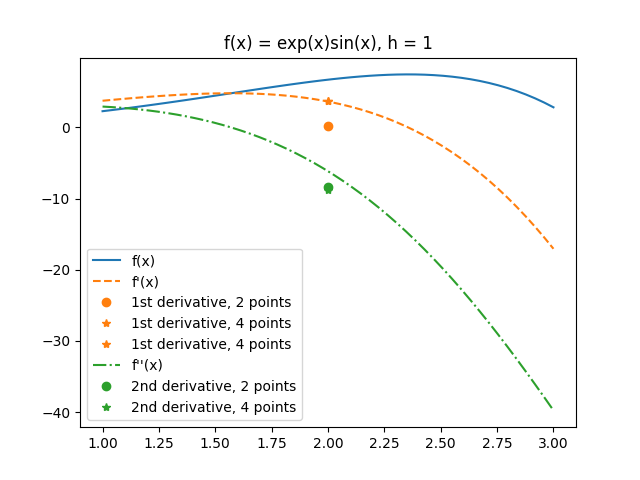
\includegraphics[width=.8\textwidth]{q4.png}
  \captionof{figure}{Aproximação para 1a e 2a derivada.}
  \label{fig:q4}
\end{figure}
Considerando, por exemplo, $h=\Delta x = 1$ e
utilizando a aproximação obtida na Eq.\eqref{eq:leveque_coeffs} para $f'(x=2)$
e $f''(x=2)$, obtemos os seguintes valores para os casos solicitados

(i) Central com 2 e 3 pontos
obtemos os coeficientes 


(ii) Central com 4 e 5 pontos

caso desejemos plotar a dependência do erro de aproximação com relação ao passo dediscretização $h$, vide Fig.~\ref{fig:q4_error}, percebemos que as aproximações com mais pontos, 3 pontos para a primeira derivada e 5 pontos para a segunda, resultam em um erro menor independente do valor de $h$. Além disso, percebe-se que o valor de $h$ influencia positivamente o erro, com menores valores de $h$ resultando em erros menores, efeito observado independente do número de pontos.
\begin{figure}[h]
  \centering
  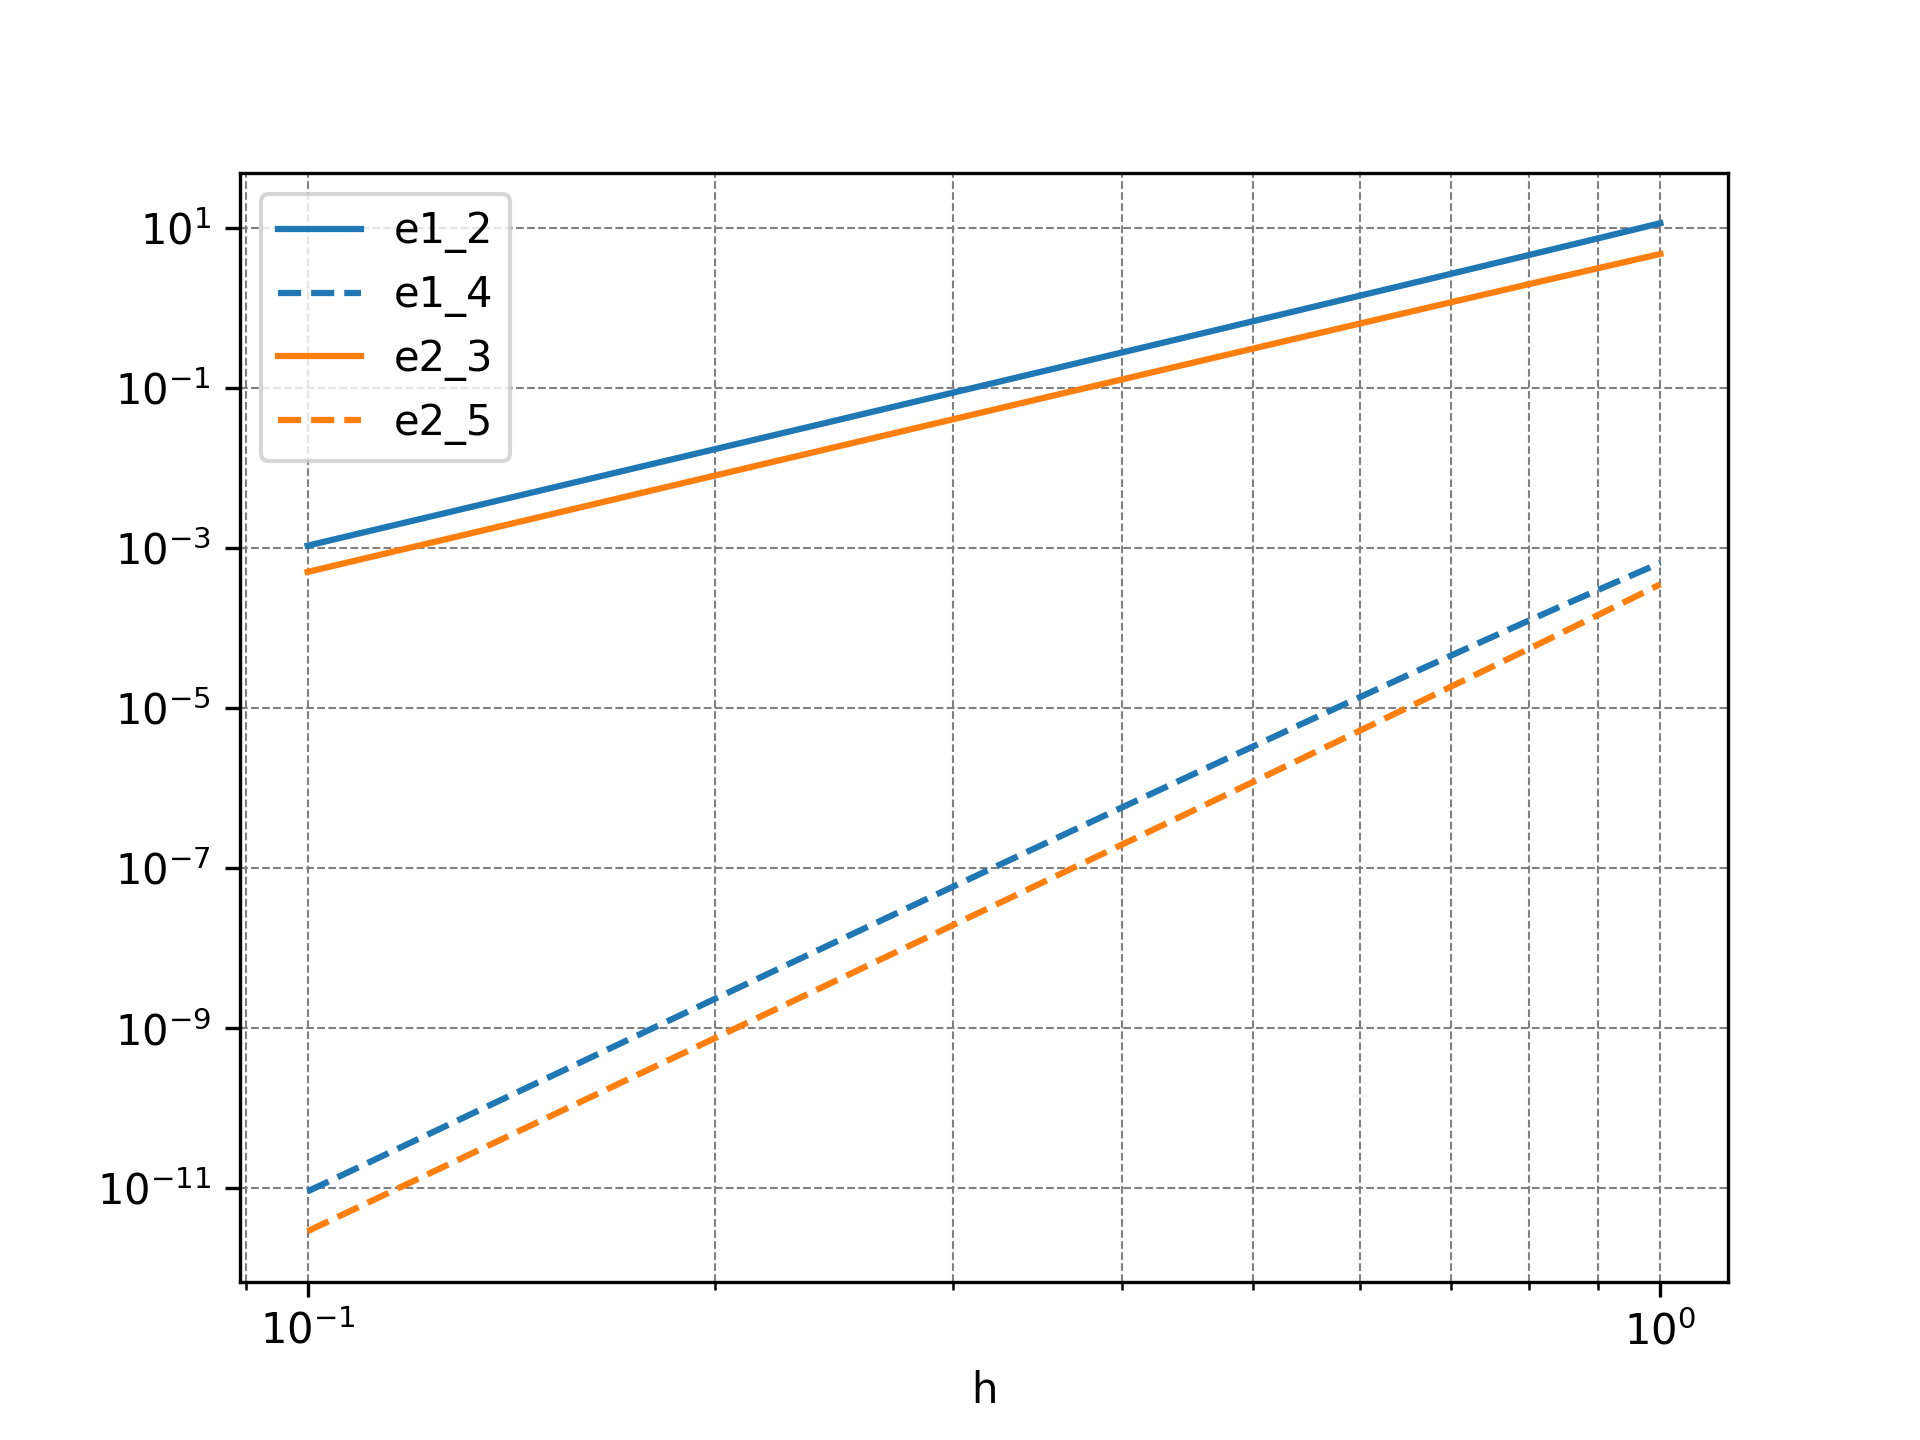
\includegraphics[width=.8\textwidth]{q4_error.png}
  \captionof{figure}{Evolução do erro de aproximação com variação de $h$.}
  \label{fig:q4_error}
\end{figure}

\begin{thebibliography}{9}
\bibitem{leveque}
Randall J. LeVeque (2007) \emph{Finite Difference Methods for Ordinary and Partial Differential Equations:
Steady-State and Time-Dependent Problems}, Society for Industrial and Applied Mathematics 
\end{thebibliography}
\end{document}
